%%% In this section, you will describe all of the various artifacts that you will generate and maintain during the project life cycle. Describe the purpose of each item below, how the content will be generated, where it will be stored, how often it will be updated, etc. Replace the default text for each section with your own description. Reword this paragraph as appropriate.

\subsection{Major Documentation Deliverables}
These deliverables are major grade components of the course. Completing these documents should generally be the sprint goal during the applicable sprint period. Refer to current and previous course syllabi and schedules to estimate the due dates of these items. Remove this explanatory paragraph from your draft, but leave the heading.

\subsubsection{Project Charter}
Describe how this document will be maintained and updated (how often, under what circumstances, etc.). When will the initial version be delivered? When will the final version be delivered?

\subsubsection{System Requirements Specification}
Describe how this document will be maintained and updated (how often, under what circumstances, etc.). When will the initial version be delivered? When will the final version be delivered?

\subsubsection{Architectural Design Specification}
Describe how this document will be maintained and updated (how often, under what circumstances, etc.). When will the initial version be delivered? When will the final version be delivered?

\subsubsection{Detailed Design Specification}
Describe how this document will be maintained and updated (how often, under what circumstances, etc.). When will the initial version be delivered? When will the final version be delivered?

\subsection{Recurring Sprint Items}

\subsubsection{Product Backlog}
Items will be added to the product backlog based on the Software Requirements Specification (SRS). The items will be prioritized based on their importance and complexity, which will be discussed by the members of the team, with the final decision being made by a group vote. To maintain and share the product backlog, software such or Excel or Jira may be used.

\subsubsection{Sprint Planning}
Each sprint will be planned by the end of a sprint, where the team will review the updates on the product backlog, prioritize new items, and establish sprint goals. There will be 8 sprints total, with the first 4 being in Senior Design 1 (CSE 4316-002) and the last 4 being in the following semester Senior Design 2 (CSE 4317-002).

\subsubsection{Sprint Goal}
The sprint goal will be decided in collaboration by the team, and the team will work closely with the customer to get input. The customer will be involved in this process to ensure that the sprint goals meet with the project objects and customer expectations.

\subsubsection{Sprint Backlog}
The sprint backlog will be derived from the product backlog, with items being selected based on their priority on how they match the sprint goal. This process will be discussed and decisions will be made by the group. The sprint backlog will be maintained using collaboration software such as Excel or Jira.

\subsubsection{Task Breakdown}
Individual tasks will be assigned from the sprint backlog through team members volunteering to take them or assignment by the product owner. Time spent on tasks will be documented by the team members regularly through the chosen collaboration software to ensure accountability.

\subsubsection{Sprint Burn Down Charts}
The burn down charts will be generated each sprint by one of the team members, with each team member taking a turn to generate the chart. The total amount of effort expended by each individual team member will be accessed by the documented time data through the chosen collaboration software. The burn down charts will follow the graphing format in the example pictured below: 


\begin{figure}[h!]
    \centering
    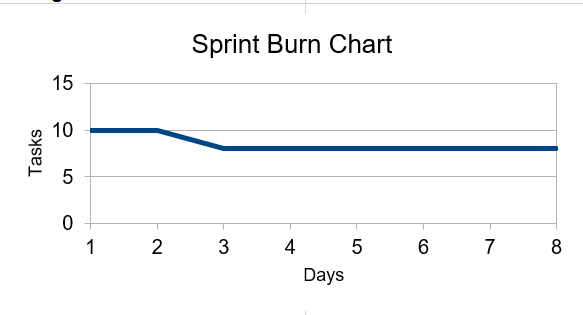
\includegraphics[width=0.5\textwidth]{images/example_burn_chart.png}
    \caption{Example sprint burn down chart}
\end{figure}

\subsubsection{Sprint Retrospective}
The sprint retrospective will occur after each sprint. The team will meet and discuss by one week of the sprint ending if the goals were met and if there was anything that could be improved. The team will document group feedback, while each team member will document their self analysis. The retrospectives will be due by a date discussed by the team.

\subsubsection{Individual Status Reports}
Status reports will be made by each team member each week for the team. Key items contained in the reports will outline their progress, completed items, and blockers.

\subsubsection{Engineering Notebooks}
Team members will update their engineering notebooks at least once a week, with each entry being at least 1 page. Team members will keep each other accountable by sharing their entries, with one designated team member each week signing off on the entries.

\subsection{Closeout Materials}
The following materials, in addition to major documentation deliverables, will be provided to the customer upon project closeout. Remove this paragraph from your draft, but leave the heading.

\subsubsection{System Prototype}
What will be included in the final system prototype? How and when will this be demonstrated? Will there be a Prototype Acceptance Test (PAT) with your customer? Will anything be demonstrated off-site? If so, will there be a Field Acceptance Test (FAT)?

\subsubsection{Project Poster}
What will be included on the poster, what will be the final dimensions, and when will it be delivered?

\subsubsection{Web Page}
What will be included on the project web page? Will it be accessible to the public? When will this be delivered? Will it be updated throughout the project, or just provided at closeout (at a minimum, you need to provide a simple web page at the end).

\subsubsection{Demo Video}
What will be shown in the demo video(s)? Will you include a B-reel footage for future video cuts? Approximately how long will the video(s) be, and what topics will be covered?

\subsubsection{Source Code}
How will your source code be maintained? What version control system will you adopt? Will source code be provided to the customer, or binaries only? If source code is provided, how will it be turned over to the customer? Will the project be open sourced to the general public? If so, what are the license terms (GNU, GPL, MIT, etc.). Where will the license terms be listed (in each source file, in a single readme file, etc.).

\subsubsection{Source Code Documentation}
What documentation standards will be employed? Will you use tools to generate the documentation (Doxygen, Javadocs, etc.). In what format will the final documentation be provided (PDF, browsable HTML, etc.)?

\subsubsection{Hardware Schematics}
Will you be creating printed circuit boards (PCBs) or wiring components together? If so, list each applicable schematic and what sort of data it will contain (PCB layout, wiring diagram, etc.). If your project is purely software, omit this section.

\subsubsection{CAD files}
Will the project involve any mechanical design, such as 3D printed or laser-cut parts? If so, what software will you use to generate the files and what file formats will you provide in your closeout materials (STL, STEP, OBJ, etc.). If your project is purely software, omit this section.

\subsubsection{Installation Scripts}
How will the customer deploy software to new installations? Will you provide installation scripts, install programs, or any other tools to improve the process? Will there be multiple scripts provided (perhaps separate scripts for the graphical front end and back end server software)? 

\subsubsection{User Manual}
Will you customer need a printed or digital user manual? Will they need a setup video? Decide now what will be provided and discuss.
